\documentclass[bachelor, och, labwork]{shiza}

\usepackage[utf8]{inputenc}
\usepackage{graphicx}

\usepackage[sort,compress]{cite}
\usepackage{amsmath}
\usepackage{amssymb}
\usepackage{amsthm}
\usepackage{fancyvrb}
\usepackage{longtable}
\usepackage{array}
\usepackage[english,russian]{babel}
\usepackage{minted}

\usepackage{tempora}


% \usepackage[colorlinks=false]{hyperref}


\newcommand{\eqdef}{\stackrel {\rm def}{=}}


\begin{document}

\title{Алгоритмы алгебры и теории чисел}

\course{4}

\group{431}

\napravlenie{10.05.01 "--- Компьютерная безопасность}


\author{Никитина Арсения Владимировича}


\satitle{доцент}
\saname{А.\,С.\,Гераськин}


\date{2022}

\maketitle

% Включение нумерации рисунков, формул и таблиц по разделам
% (по умолчанию - нумерация сквозная)
% (допускается оба вида нумерации)
%\secNumbering


\tableofcontents

\section{Задание лабораторной работы}

Реализовать факторизацию Ферма.

\section{Теоретическая часть}

Метод Ферма основан на теореме о представлении числа в виде разности двух квадратов:

Если $n>1$ нечётно, то существует взаимно однозначное соответствие между разложением 
$n=a\cdot b$ и представлением в виде разности квадратов $n=x^{2}-y^{2}$ с $x>y>0$,
задаваемое формулами $x=(a+b)/2,$ $y=(a-b)/2,$ $a=x+y$, $b=x-y.$

Для разложения на множители нечётного числа $n$ ищется пара чисел $(x,y)$ таких, 
что $x^2 - y^2 = n$, или $(x-y)\cdot (x+y)=n$. При этом числа $(x+y)$ и $(x-y)$ 
являются делителями $n$, возможно, тривиальными (то есть одно из них равно 1, а 
другое --- $n$.

В нетривиальном случае равенство $x^2 - y^2 = n$ равносильно $x^{2}-n=y^{2}$, 
то есть тому, что $x^{2}-n$ является квадратом.

Поиск квадрата такого вида начинается с $x=\left\lceil {\sqrt {n}}\right\rceil$ --- 
наименьшего числа, при котором разность $x^{2}-n$ неотрицательна.

Для каждого значения $k\in \mathbb  {N}$, начиная с $k=1$, вычисляют 
$\left(\left\lceil {\sqrt {n}}\right\rceil +k\right)^{2}-n$ и проверяют, не 
является ли это число точным квадратом. Если не является, то $k$ увеличивают на 
единицу и переходят на следующую итерацию.

Если $\left(\left\lceil {\sqrt {n}}\right\rceil +k\right)^{2}-n$ является 
точным квадратом, то есть $x^{2}-n=\left(\left\lceil {\sqrt {n}}\right\rceil +k\right)^{2}-n=y^{2},$
то получено разложение:

$n=x^{2}-y^{2}=(x+y)(x-y)=a\cdot b,$

в котором $\displaystyle x=\left\lceil {\sqrt {n}}\right\rceil +k.$

Если оно является тривиальным и единственным, то $n$ --- простое.

На практике значение выражения на $(k+1)$-м шаге вычисляется с учётом значения 
на $k$-м шаге:

$(s+1)^{2}-n=s^{2}+2s+1-n,$
где $s=\left\lceil {\sqrt {n}}\right\rceil +k.$


\section{Практическая часть}
\subsection{Пример работы алгоритма}
\begin{figure}[H]
    \centering
    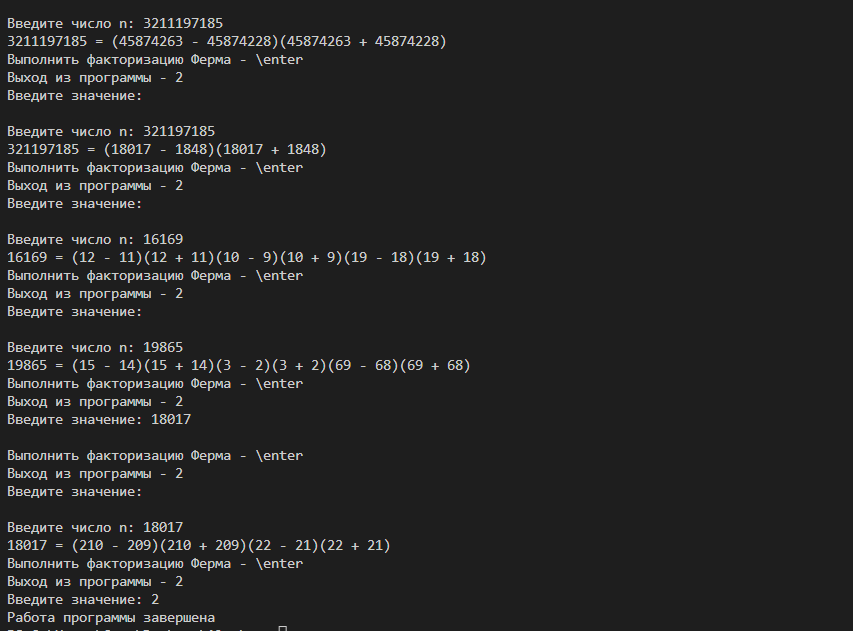
\includegraphics[width=1\textwidth]{pic1.png}
    \caption{}
\end{figure}

\setminted[python]{linenos,breaklines=true, fontsize=\small, style=bw}
    \subsection{Код программы, реализующей рассмотренный алгоритм}
        \inputminted{python}{lab11.py}

\end{document}